\chapter{Диэлектрические волноводы}

Рассмотрим оптически более плотный волновод в среде. В силу явления полного внутреннего отражения в нём может распространяться волна:

\begin{center}
	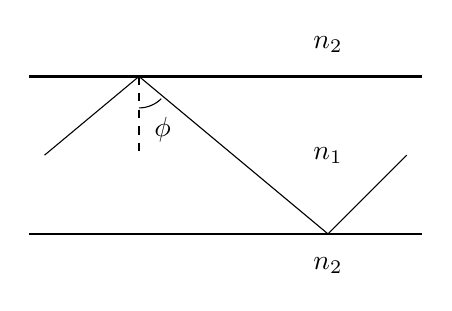
\begin{tikzpicture}[scale=0.2]
		\draw[thick] (-10, 10) -- (15,10);
		\draw[thick] (-10, 0) -- (15,0);
		\draw (-9, 5) -- (-3, 10) -- (9, 0) -- (14, 5);
		\draw[dashed] (-3, 10) -- (-3, 5);
		\draw (-3, 8) arc (-90:-45:2 and 2);
		\node[below] at (-1.5, 8) {$\phi$};
		\node at (9, 12) {$n_2$};
		\node at (9, 5) {$n_1$};
		\node at (9, -2) {$n_2$};
	\end{tikzpicture}
\end{center}

\[
	\phi \ge \phi_\mathrm{min},\quad \sin\phi_\mathrm{min} = n_1 / n_2.
\]

При таких переотражениях получается волна, распространяющаяся вдоль волновода.

Фазовая скорость волны равна
\[
	v_p = \frac{u_2}{\sin\phi} \le u_1,
\]
\[
	u_1 \ge v_p \ge u_2.
\]

Угол \( \phi \) падения связан с размерами и частотой волны. Если \( \phi < \phi_\mathrm{min} \), то волна рассеивается в окружающее пространство. Следовательно, получается отсечка.

\[
	h^2 = k_1^2 - g_1^2 = k_2^2 - g_2^2.
\]
\[
	g_2^2 > 0,\ g_1^2 < 0,
\]
\[
	g_1 = iq,\ g_2 = g.
\]

\[
	\eps_1\mu_1\omega^2 + q^2 = \eps_2\mu_2\omega^2 - g^2.
\]
Пусть \( a \) -- характерный размер волновода, тогда
\[
	\overline{g} = ag,\quad \overline{q} = aq,
\]
\[
	\overline{q}^2 + \overline{g}^2 = a^2\omega^2\eps_1\mu_1(\overline{\eps}\overline{\mu} - 1) = \overline{k}_1^2(\overline{\eps}\overline{\mu} - 1) = \overline{R}^2.
\]
\(\overline{R}\) -- нормированная частота.

Рассмотрим плоский волновод:
\[
	\Delta_\perp E_{z1} + g^2 E_{z1} = 0,
\]
\[
	\Delta_\perp E_{z2} - q^2 E_{z2} = 0,
\]
при граничном условии
\begin{align*}
	E_{z1}(x=a) = E_{z2}(x=a),\\
	E_{z1}(x=-a) = E_{z2}(x=-a),\\
	H_{y1}(x=a) = H_{y2}(x=a),\\
	H_{y1}(x=-a) = H_{y2}(x=-a).
\end{align*}

\begin{align*}
	E_{z1} = A_1\cos(gx) + B_1\sin(gx),\\
	E_{z2} = A_2 e^{-qx} + B_2 e^(qx).\\
\end{align*}

Поперечные поля имеют вид
\begin{align*}
	E_{x1} = -\frac{ih}{g}(-A_1\sin gx + B_1\cos gx),\\
	H_{y1} = -\frac{i\omega\eps_1}{g}(-A_1\sin gx + B_1\cos gx)\\
\end{align*}

Если \(A_1 = 0\), то волны называют чётными (e), \( B_1 = 0 \) -- нечётными (o).

Во второй области
\begin{align*}
	E_{x2} = \frac{ih}{q}(-A_2 e^{-qx} + B_2 e^{qx}),\\
	H_{y2} = \frac{i\omega\eps_2}{q}(-A_2 e^{-qx} + B_2 e^{qx})\\
\end{align*}

В полупространстве \( x>0 \) в силу конечности поля на бесконечности
\[
	E_{x2} = -\frac{ih}{q} A_2 e^{-qx},\quad
	H_{y2} = -\frac{i\omega\eps_2}{q} A_2 e^{-qx}
\]

Сшиваем чётную волну:
\[
	B_1\sin ga = A_2e^{-qa},\quad -\frac{\eps_1}{g} B_1\cos ga = -\frac{\eps_2}{q} A_2 e^{-qa},
\]
\[
	\tg ga = \frac{\eps_1}{\eps_2}\cdot\frac{q}{g}.
\]

Для нечётных
\[
	\ctg ga = -\frac{\eps_2}{\eps_1}\cdot\frac{q}{g}.
\]

Тут картинки с графическим решением дисперсионных уравнений.

Теперь H-волны:
\[
	H_{z1} = A_1 \cos gx + B_1 \sin gx,\quad H_{z2} = A_2 e^{-gx} + B_2 e^{gx}
\]
поперечные поля
\begin{align*}
	E_{y1} = \frac{i\omega\mu}{g}(-A_1\sin gx + B_1\cos gx),\\
	H_{x1} = \frac{-ih}{g}(-A_1\sin gx + B_1\cos gx),
\end{align*}

\begin{align*}
	E_{y2} = \frac{-i\omega\mu}{q}(-A_2 e^{-gx} + B_2 e^{gx}),\\
	H_{x2} = \frac{ih}{q}(-A_2 e^{-qx} + B_2 e^{qx}),
\end{align*}

Рассмотрим снова то же полупространство (\( B_2 = 0 \)) и граничные условия
\begin{align*}
	\mu_1H_{x1}(x=a) = \mu_2H_{x2}(x=a),\\
	H_{z1}(x=a) = H_{z2}(x=a),\\
\end{align*}

Чётные волны (\( A_1 = 0 \))
\begin{align*}
	\frac{\mu_1}{g}B_1\cos ga = -\frac{\mu_2}{q}(-A_2 e^{-qa}),\\
	B_1 \sin gx = A_2 e^{-qx},\\
\end{align*}
откуда
\[
	\frac{\mu_1}{g}\cos ga = \frac{\mu_2}{q}\sin ga
\]
\[
	\tg ga = \frac{\mu_1}{\mu_2}\cdot\frac{q}{g}
\]
Для нечётных
\[
	\ctg ga = -\frac{\mu_2}{\mu_1}\cdot\frac{q}{g}.
\]

Коэффициент замедления
\[
	n = \frac{u}{v_p},\quad n_{max} = \frac{u_2}{u_1}.
\]

Для круглого диэлектрического волновода как E- и H- волны можно рассматривать только волны \( E_{0n}, H_{0n} \). В общем случае наблюдаются гибридные волны:
\begin{align*}
	& \Delta_\perp E_{z1} + g^2 E_{z1} = 0,\\
	& \Delta_\perp H_{z1} + g^2 H_{z1} = 0,\\
	& \Delta_\perp E_{z2} - q^2 E_{z2} = 0,\\
	& \Delta_\perp H_{z2} - q^2 H_{z2} = 0,\\
\end{align*}

\begin{center}
	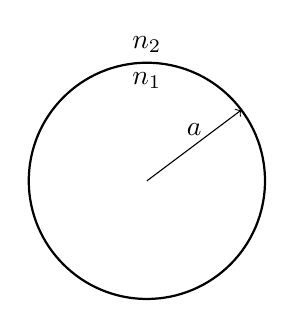
\begin{tikzpicture}[scale=0.15]
		\draw[thick] (0,0) circle (10);
		\draw[->] (0,0) -- (8, 6);
		\node[above] at (4, 3) {$a$};
		\node[above] at (0, 10) {$n_2$};
		\node[below] at (0, 10) {$n_1$};
	\end{tikzpicture}
\end{center}

\[
	\left.E_{z2}\right|_{r\to\infty} \to 0,\quad
	\left.H_{z2}\right|_{r\to\infty} \to 0,
\]

И ещё граничные условия
\begin{align*}
	& \left.E_{z1}\right|_{r=a} = \left.E_{z2}\right|_{r=a},\\
	& \left.H_{z1}\right|_{r=a} = \left.H_{z2}\right|_{r=a},\\
	& \left.E_{\alpha1}\right|_{r=a} = \left.E_{\alpha2}\right|_{r=a},\\
	& \left.H_{\alpha1}\right|_{r=a} = \left.H_{\alpha2}\right|_{r=a},\\
\end{align*}

Решения имеют вид:
\begin{align*}
	& E_{z1} = E_1 J_m(gr)e^{im\alpha},\\
	& H_{z1} = H_1 J_m(gr)e^{im\alpha},\\
	& E_{z2} = E_2 K_m(qr)e^{im\alpha},\\
	& H_{z2} = H_2 K_m(qr)e^{im\alpha},\\
\end{align*}

Теперь выразим граничные условия:
\begin{align*}
	& E_1 J_m(ga) = E_2 K_m(qa),\\
	& H_1 J_m(ga) = H_2 K_m(qa),\\
	& \frac{-1}{g^2}\left(\frac{imh}{r}E_1 J_m(ga) -
	\mu_1\omega g H_1 J_m'(ga)\right) =
	\frac{1}{q^2}\left(\frac{imh}{r}E_2 K_m(qa) -
	\mu_2\omega q H_2 K_m'(qa)\right),\\
	& \frac{-1}{g^2}\left(\omega\eps_1 g E_1 J_m'(ga) + \frac{h}{a}im H_1 J_m(ga)\right) = \frac{1}{q^2}\left(\omega\eps_2 q E_2 K_m'(qa) + \frac{h}{a}im H_2 K_m(qa)\right).
\end{align*}

Эта система имеет нетривиальное решение только если её определитель равен нулю:
\[
	\begin{vmatrix}
		J_m(ga) & 0 & -K_m(qa) & 0 \\
		0 & J_m(ga) & 0 & -K_m(qa) \\
		\frac{-imh}{ag^2}J_m(ga) & \frac{\mu_1\omega}{g}J_m'(ga) & \frac{-imh}{aq^2}K_m(qa) & \frac{\mu_2\omega}{q}K_m'(qa)\\
		\frac{-\omega\eps_1}{g}J_m'(ga) & \frac{-imh}{g^2}J_m(ga) & \frac{-\omega\eps_2}{q}K_m'(ga) & \frac{-imh}{q^2}K_m(ga)\\
	\end{vmatrix} = 0.
\]

Введём пару вспомогательных функций
\[
	s_m(x) = \frac{J_m'(x)}{xJ_m(x)},\quad
	t_m(x) = -\frac{K_m'(x)}{xK_m(x)}
\]
и перепишем определитель в виде
\[
	\begin{vmatrix}
		1 & 0 & -1 & 0 \\
		0 & 1 & 0 & -1 \\
		\frac{-imh}{ag^2} & a\mu_1\omega s_m(ga) & \frac{-imh}{aq^2} & -a\mu_2\omega t_m(qa)\\
		-a\omega\eps_1 s_m(ga) & \frac{-imh}{g^2} & a\omega\eps_2t_m(ga) & \frac{-imh}{q^2}\\
	\end{vmatrix} = 0.
\]
\[
	-\left(\frac{mh(g^2 + q^2)}{ag^2q^2}\right)^2 + a^2\omega^2(\eps_1s_m(ga) - \eps_2t_m(qa))(\mu_1 s_m(ga) - \mu_2 t_m(qa)) = 0.
\]

\begin{problem}
Определить толщину диэлектрической пластины, при которой коэффициент замедления для волны \(E_0\) на частоте 10 ГГц равен \( 1,\!2 \), \(\overline{\eps} = 2,\!5\).
\end{problem}

\[
	n = \frac{c}{v_p} = \frac{ch}{\omega},
\]
\[
	h^2 = \omega^2/c^2 + q^2 = \overline{\eps\mu}\omega^2/c^2 - g^2,
\]
\[
	q = \sqrt{n^2 - 1}\omega/ c
\]
\[
	g = \sqrt{\overline{\eps\mu} - n^2}\omega / c.
\]
\[
	a = \frac{1}{g}\arctg{\overline{\eps}\sqrt{\frac{n^2-1}{\overline{\eps\mu} - n^2}}}
\]
\[
	d = 2a = 6\cdot10^{-2}~\text{м}.
\]
